\subsection{Zasada prawej ręki}

\subsection{Sprawdzenie czy dwa odcinki się przecinają}
Przypuśćmy, że dysponujemy przestrzenią $\mathbb{R}^3$ oraz odcinkami danymi przez pary punktów 
$(P_1, P_2)$ oraz $(P_3, P_4)$. Naszym celem będzie sprawdzenie
czy istnieje punkt wspólny pomiędzy tymi odcinkami.

Na początku omówmy geometryczną interpretację iloczynów skalarnych, którą wykorzystamy w dalszych rozważaniach.

Dane są wektory $\vec{u},\vec{v} \in \mathbb{R}^2$ oraz prosta $L$ prostopadła
do $\vec{u}$ przechodząca przez punkt $(0,0)$. Wtedy iloczyn skalarny 
standardowy $\vec{u} \cdot \vec{v}$
jest 
\begin{itemize}[]
	\item dodatni jeśli groty $\vec{u}$ oraz $\vec{v}$ są po tej samej stronie płaszczyzny podzielonej przez prostą $L$,
	\item ujemny jeśli groty $\vec{u}$ oraz $\vec{v}$ są po  przeciwnych stronach płaszczyzny podzielonej przez prostą $L$,
	\item zerowy w przypadku kiedy wektor $\vec{v}$
	leży na prostej $L$.
\end{itemize}

Teraz możemy sformuować uogólnienie zasady prawej ręki.
Dane są wektory $\vec{u},\vec{v},\vec{w} \in \mathbb{R}^3$.
Wtedy jeśli $(\vec{u} \times \vec{v})
\cdot (\vec{u} \times \vec{w}) > 0$, to bazy
$(\vec{u}, \vec{v},  (\vec{u} \times \vec{v}))$ oraz
$(\vec{u}, \vec{w},  (\vec{u} \times \vec{w}))$ są zgodne
co interpretujemy geometrycznie, jako sytuację, w której 
groty wektorów 
$\vec{v}, \vec{w}$ są po tej samej stronie względem prostej,
na której leży wektor $\vec{u}$.


Pomysł na algorytm polega na sprawdzeniu czy punkty $P_1$
oraz $P_2$ znajdują po przeciwnych stronach prostej 
przechodzącej przez punkty $P_3$ i $P_4$ oraz 
na sprawdzeniu czy punkty $P_3$
oraz $P_4$ znajdują po przeciwnych stronach prostej 
przechodzącej przez punkty $P_1$ i $P_2$. Jeśli odpowiedź
na tak postawione pytanie jest twierdząca, to zadane
odcinki muszą się przecinać.


\begin{algorithm}[H]
	\caption{Sprawdzenie, czy dwa odcinki się przecinają w przestrzeni $\mathbb{R}^3$}
	\begin{algorithmic}[1]
		\Procedure{SegmentIntersectionR3($P_1$, $P_2$, $P_3$, $P_4$)}{}
		\If{$P_1 = P_3$ lub $P_1 = P_4$ lub $P_2 = P_3$ lub $P_2 = P_4$}
		\State \Return \textit{true}
		\EndIf
		\State $\vec{v}_{12} \gets P_2 - P_1$
		\State $\vec{v}_{34} \gets P_4 - P_3$
		\State $\vec{w} \gets \vec{v}_{12} \times \vec{v}_{34}$	
		\If{$\vec{w} = \mathbf{0}$} \Comment Jeśli odcinki są współliniowe
		\State $d \gets \max\{|P_1P_3|, |P_1P_4|, |P_2P_3|, |P_2P_4|\}$
		\If{$d \leq |P_1P_2| + |P_3P_4|$}
		\State \Return \textit{true}
		\EndIf
		\EndIf
		\State $\vec{v}_{13} \gets P_3 - P_1$
		\State $\vec{v}_{14} \gets P_4 - P_1$
		\If{$(\vec{v}_{12} \times \vec{v}_{14}) \cdot \vec{w}$ oraz 
		$(\vec{v}_{12} \times \vec{v}_{13}) \cdot \vec{w}$ są tego samego znaku}
		\State \Return \textit{false}
		\EndIf
		\State $\vec{v}_{32} \gets P_2 - P_3$
		\State $\vec{v}_{31} \gets P_1 - P_3$
		\If{$(\vec{v}_{34} \times \vec{v}_{31}) \cdot \vec{w}$ oraz 
		$(\vec{v}_{34} \times \vec{v}_{32}) \cdot \vec{w}$ są tego samego znaku}
		\State \Return \textit{false}
		\EndIf
		\State \Return \textit{true}
		\EndProcedure
	\end{algorithmic}
	\label{segment_intersection_r3}
\end{algorithm}

Zauważmy, że gdybyśmy powyższy problem rozwiązywali w przestrzeni $\mathbb{R}^2$,
to podczas badania iloczynów wektorowych, jedyne co nas by interesowało
to znak 3-ej współrzędnej. Z zasady prawej ręki, jeśli
trzecia współrzędna wektora 
$\vec{u} \times \vec{v}$ jest dodatnia, to wektor $\vec{v}$
znajduje się po lewej stronie wektora $\vec{u}$ oraz jeśli 
jest ujemna to wektor $\vec{v}$
znajduje się po prawej stronie wektora $\vec{u}$. 

Fakt ten znacznie upraszcza sprawdzanie orientacji wektorów iloczynem wektorowym.

Trzecią współrzędną iloczynu wektorowego $\vec{u} \times \vec{v}$ w $\mathbb{R}^2$
obliczymy korzystając ze wzoru
\[c = \vec{u}_x \vec{v}_y - \vec{v}_x \vec{u}_y.\]



\begin{algorithm}[H]
	\caption{Sprawdzenie, czy dwa odcinki się przecinają w przestrzeni $\mathbb{R}^2$}
	\begin{algorithmic}[1]
		\Procedure{Prod2($\vec{u}$,$\vec{v}$)}{}
		\State \Return $\vec{u}_x \vec{v}_y - \vec{v}_x \vec{u}_y$
		\EndProcedure
		\Procedure{SegmentIntersectionR2($P_1$, $P_2$, $P_3$, $P_4$)}{}
		\If{$P_1 = P_3$ lub $P_1 = P_4$ lub $P_2 = P_3$ lub $P_2 = P_4$}
		\State \Return \textit{true}
		\EndIf
		\State $\vec{v}_{12} \gets P_2 - P_1$
		\State $\vec{v}_{34} \gets P_4 - P_3$
		\If{Prod2$(\vec{v}_{12}$, $\vec{v}_{34}) = 0$} \Comment Jeśli odcinki są współliniowe
		\State $d \gets \max\{|P_1P_3|, |P_1P_4|, |P_2P_3|, |P_2P_4|\}$
		\If{$d \leq |P_1P_2| + |P_3P_4|$}
		\State \Return \textit{true}
		\EndIf
		\EndIf
		\State $\vec{v}_{13} \gets P_3 - P_1$
		\State $\vec{v}_{14} \gets P_4 - P_1$
		\If{$\text{Prod2}(\vec{v}_{12}$, $\vec{v}_{14})$ $\cdot$ $\text{Prod2}(\vec{v}_{12}$, $\vec{v}_{13}) > 0$}
		\State \Return \textit{false}
		\EndIf
		\State $\vec{v}_{32} \gets P_2 - P_3$
		\State $\vec{v}_{31} \gets P_1 - P_3$
		\If{$\text{Prod2}(\vec{v}_{34}$, $\vec{v}_{31})$ $\cdot$ $\text{Prod2}(\vec{v}_{34}$, $\vec{v}_{32}) > 0$}
		\State \Return \textit{false}
		\EndIf
		\State \Return \textit{true}
		\EndProcedure
	\end{algorithmic}
	\label{segment_intersection_r2}
\end{algorithm}


\subsection{Problem przynależności punktu do wielokąta}


\subsection{,,Metoda zamiatania''}
\subsubsection{Znajdowanie długości sumy odcinków}
Mamy zbiór być może nakładających się odcinków w jednowymiarowej przestrzeni Euklidesowej, które siłą rzeczy
znajdują się na jednej prostej. Naszym zadaniem jest policzyć długość tych odcinków, ale w ten sposób, że jeśli jakiś
fragment przestrzeni należy do więcej niż jednego odcinka, to i tak liczymy go tylko raz (czyli liczymy pole sumy
teoriomnogościowej tych odcinków).

Aby rozwiązać ten problem skorzystamy z metody zamiatania. Dla
uproszczenia przyjmijmy, że odcinki z wejściowego zbioru $X$ są reprezentowane
jako dwuwymiarowe punkty, takie, że dla każdego punktu, $x$-owa
współrzędna jest taka sama.

W ogólności w przestrzeni mamy kilka serii
nakładających się odcinków (zanim jeden odcinek się skończy, to już się zaczyna inny). Gdy poznamy długość każdej
z takich serii, odpowiedzią będzie suma ich długości. Musimy wykryć, gdzie taka pojedyncza seria się zaczyna, a gdzie
kończy, czyli mieć jej zakres. Zakres da nam długość.

Idea rozwiązania polega na przejściu miotłą od najmniejszego względem 
$y$-owej współrzędnej punktu w górę. Podczas przechodzenia
będziemy kontrolować liczbę odcinków, które są w kontakcie z miotłą.

Jako, że nie możliwym jest przechodzenie w sposób ciągły, w
metodzie zamiatania rozważamy tzw. \textit{zdarzenia}, które pozwalają
sprowadzić ten problem do problemu dyskretnego.

W naszym przypadku, każde natrafienie miotły na dowolny punkt
traktujemy jako zdarzenie. Jeśli dojdzie do takiego zdarzenia
zapiszemy współrzędną $y$ oraz informację czy punkt zaczyna, czy też
kończy jakiś odcinek.

W algorytmie \ref{VerticalSegmentsUnionLength} przyjmujemy, że
struktura Event składa się ze zmiennej Coord, która reprezentuje
współrzędną $y$ oraz zmiennej IsStartingPoint, która 
reprezentuje informację, czy punkt zaczyna odcinek.

\begin{algorithm}[H]
	\caption{Znajdowanie długości sumy odcinków}
	\begin{algorithmic}[1]
		\Procedure{VerticalSegmentsUnionLength}{$X$}
		\State Niech \textit{Events} to lista zdarzeń typu Event
		\For{$AB \in X$}
			\If{$A_y \leq B_y$}
				\State Events.PushBack($A$, \textit{true})
				\State Events.PushBack($B$, \textit{false})
			\Else
				\State Events.PushBack($A$, \textit{false})
				\State Events.PushBack($B$, \textit{true})
			\EndIf
		\EndFor
		\State Posortuj rosnąco Events względem zmiennej Coord
		\State Niech \textit{level} oznacza liczbę nałożonych na siebie odcinków w danym momencie
		\State Niech \textit{startPoint} oznacza początek ciągłej sumy odcinków
		\State Niech \textit{distance} oznacza aktualnie policzoną długość
		\For{event $\in$ Events} \Comment Ten zapis rozumiemy jako przejście od pierwszego elementu do ostatniego elementu na liście
			\If{event.IsStartingPoint}
				\If{level $= 0$}
					\State startPoint = event.Coord
				\EndIf
				\State level $\gets$ level $+$ 1
			\Else 
				\State level $\gets$ level $-$ 1
				\If{level $= 0$}
					\State distance = distance event.Coord - startPoint
				\EndIf
			\EndIf
		\EndFor
		\State \Return distance
		\EndProcedure
	\end{algorithmic}
	\label{VerticalSegmentsUnionLength}
\end{algorithm}

\subsubsection{Znajdowanie pola sumy prostokątów}
Wyobraź sobie prostokąty. Teraz wyobraź sobie pionową linię zamiatającą. Idzie ona od lewej do prawej. Tym
razem zatrzymuje się ona za każdym razem, gdy natrafi na pionowy bok prostokąta (każdy prostokąt ma dwa takie
boki). Takie zatrzymanie nazywamy zdarzeniem. 

W czasie zatrzymania obliczamy, jaka jest długość przecięcia wszystkich prostokątów z linią zamiatającą. Oznaczmy tę długość $D$. Nazwijmy ją wysokością. Teraz wiemy, że ta wysokość
nie zmieni się do następnego zdarzenia. Dlatego jeśli jedno zdarzenie zdarzyło się na współrzędnej $x_1$, a następne na
$x_2$, to pole prostokątów między tymi zdarzeniami wynosi $(x_2-x_1)\cdot D$. Suma takich pól jest szukanym polem.

W algorytmie \ref{VerticalSegmentsUnionLength} przyjmujemy, że
struktura Event składa się ze zmiennej Coord, która reprezentuje
współrzędną $y$ oraz zmiennej IsStartingPoint, która 
reprezentuje informację, czy punkt zaczyna odcinek. Ponadto 
struktura zawiera zmienną Idx, która przechowuje
indeks prostokąta w odpowiedniej tablicy.

Ponadto struktura Rectangle tworzona jest przez zmienne MinX, MinY, MaxX, MaxY.

\begin{algorithm}[H]
	\caption{Znajdowanie pola sumy prostokątów}
	\begin{algorithmic}[1]
		\Procedure{RectangleUnionArea}{rectangles -- tablica prostokątów, $n$ -- liczba prostokątów}
		\State Niech \textit{Events} to lista zdarzeń typu Event
		\For{$i \in 1,2 \ldots, n$}
		\State Events.PushBack(rectangles$[i]$.MinX, \textit{true}, $i$)
		\State Events.PushBack(rectangles$[i]$.MaxX, \textit{false}, $i$)
		\EndFor
		\State Posortuj rosnąco Events względem zmiennej Coord
		\State Niech \textit{currentSegments} oznacza 
		\State Niech \textit{startPoint} oznacza początek ciągłej sumy odcinków
		\State Niech \textit{area} oznacza aktualnie policzone pole
		
		\For{event $\in$ Events} \Comment Ten zapis rozumiemy jako przejście od pierwszego elementu do ostatniego elementu na liście
		\If{currentSegments.Count > 0}
		\State distance $\gets$  VerticalSegmentsUnionLength(currentSegments)
		\State area $\gets$ area $+$  distance $\cdot$ (event.Coord - startPoint)
		\EndIf
		\State startPoint = event.Coord
		\State $A = (0, \text{rectangles}[\text{event.Idx}].\text{MinY})$
		\State $B = (0, \text{rectangles}[\text{event.Idx}].\text{MaxY})$
		\If{event.IsStartingPoint}
		\State currentSegments.Add($AB$)
		\Else
		\State currentSegments.Remove($AB$)
		\EndIf
		\EndFor
		
		\State \Return area
		\EndProcedure
	\end{algorithmic}
	\label{RectangleUnionArea}
\end{algorithm}

\subsubsection{Sprawdzenie czy w zbiorze odcinków istnieją przecinające się odcinki}
Problem ten rozważamy w przestrzeni $\mathbb{R}^2$, bardzo pomocny będzie 
algorytm \ref{segment_intersection_r2}, który roztrzyga, czy dwa odcinki
w przestrzeni $R^2$ przecinają się. Ponadto przy drugim wariancie założymy,
że dysponujemy funkcją, która znajduje punkt wspólny dwóch 
przecinających się odcinków. 

\textbf{Dane:} Zbiór odcinków $S$, taki, że nie istnieją 3 wierzchołki przecinające
się w tym samym punkcie oraz nie istnieją odcinki pionowe.

\textbf{Wariant 1:} Roztrzygnięcie, czy w zbiorze wierzchołków istnieje 
para przecinających się odcinków.

\textbf{Wariant 2:} Znalezienie wszystkich punktów, które 
stanowią miejsce przecięć dwóch odcinków ze zbioru $S$.

W celu rozwiązania obu wariantów, zastosujemy metodę zamiatania. Wyobraźmy
sobie dwuwymiarową płaszczyznę, na której rozmieszczone są odcinki ze zbioru $S$.
Ustawiamy miotłę po lewej stronie tej płaszczyzny. Będziemy przechodzić do prawej strony.

Zajmijmy się teraz \textbf{wariantem 1}.

Zakładamy, że \textit{zdarzenie}, będzie przechowywać 
\begin{itemize}
	\item wierzchołek $p$, który je spowodował, 
	\item odcinek $s$, którego $p$ jest początkiem lub końcem,
	\item informację, czy $p$ jest początkiem, czy też końcem odcinka $s$,
\end{itemize}
gdzie jako początek odcinka $s$ rozumiemy wierczhołek, który jest 
mniejszy względem $x$ (czyli bardziej po lewej stronie).

Jako \textit{zdarzenie} będziemy traktowali natrafienie na punkt zaczynający 
lub kończący jakiś odcinek należący do zbioru $S$.

Przez $X$-strukturę, będziemy rozumieli strukturę danych przechowującą 
kolejne wydarzenia. Oczekujemy, że 
\begin{itemize}
	\item insert(\textit{zdarzenie})  -- wstawienie zdarzenia do struktury,
	\item findfirst(\textit{zdarzenie})  -- wyznaczenie oraz usunięcie zdarzenia
	o najmniejszej współrzędnej $x$.
\end{itemize}

Niech $s_1, s_2 \in S$ to odcinki, które w danym momencie przecinają się 
z miotłą, wtedy będziemy mówili, że $s_1 > s_2$ na tej miotle,
jeśli pozycja $y$ punktu przecięcia odcinka $s_1$ z miotłą jest wyższa 
niż pozycja $y$ punktu przecięcia odcinka $s_2$ z miotłą.

\textbf{Obserwacja 1:} Zauważmy, że jeśli dwa odcinki przecinają się, to istnieje takie położenie
miotły, w którym te odcinki sąsiadują ze sobą w powyższym liniowym porządku.

Przez $Y$-strukturę, będziemy rozumieli strukturę danych, która w sposób 
posortowany względem pozycji w osi $Y$, przetrzymuje aktualnie przecinające się 
z miotłą odcinki. Niech $s \in S$ to odcinek, wtedy
\begin{itemize}
	\item insert($s$) -- wstawienie odcinka $s$,
	\item delete($s$) -- usunięcie odcinka $s$,
	\item above($s$) -- znalezienie ,,górnego'' sąsiada odcinka $s$,
	\item below($s$) -- znalezienie ,,dolnego'' sąsiada odcinka $s$,
	\item interchange($s_1$, $s_2$) -- zmiana uporządkowania odcinków $s_1$ i $s_2$,
\end{itemize}
są złożoności $O(log(n))$. Metoda interchange jest potrzebna do drugiego wariantu 
problemu i zostanie szczegółowo omówiona w dalszej części.

Aby osiągnąć powyższe złożoności możemy skorzystać ze zrównoważonych drzew BST, czyli
drzewa AVL lub CC.

Algorytm w \textbf{wariancie 1} będzie polegał na sprawdzaniu 
czy jakieś dwa sąsiadujące odcinki na miotle spełniają założenia 
\textbf{obserwacji 1}, jeśli tak to stanowią kandydatów na przecinające 
się wierzchołki i należy sprawdzić czy się przecinają. W taki sposób
minimalizujemy liczbę sprawdzeń.

Sprawdzenie zostanie wykonane tylko wtedy, gdy dojdzie do \textit{zdarzenia},
ponieważ każde \textit{zdarzenie} generuje nową parę sąsiedzką (dwie pary w przypadku kiedy zdarzenie dotyczy punktu startowego i jedną w przypadku przeciwnym) w uporządkowanym zbiorze odcinków przecinających się z miotłą.

\begin{algorithm}[H]
	\caption{Sprawdzenie czy w zbiorze $S$ istnieją przecinające się odcinki}
	\begin{algorithmic}[1]
		\Procedure{HasIntersectingSegments}{$S$ -- zbiór odcinków spełniający założenia}
		\State $X \gets$ \textit{zdarzenia} dla każdego punktu $p$ będącego
		końcem pewnego odcinka ze zbioru $S$
		\State $Y \gets \emptyset$
		\While{$X \not = \emptyset$}
		\State \textit{zdarzenie} = $X.$findfirst()
		\State przez $s$ i $p$ oznaczamy
		kolejno odcinek oraz punkt utożsamiony ze \textit{zdarzeniem}
		\If{$p$ jest początkiem odcinika $s$}
		\If{$s$ przecina się z $Y$.above($s$) lub z $Y$.below($s$)}
		\State \Return \textit{True}
		\EndIf
		\Else
		\If{$Y$.above($s$) przecina się z $Y$.below($s$)}
		\State \Return \textit{True}
		\EndIf
		\EndIf
		\EndWhile
		\State \Return \textit{False}
		\EndProcedure
	\end{algorithmic}
	\label{HasIntersectingSegments1}
\end{algorithm}

Złożoność powyższego algorytmu jest rzędu $n\log(n)$, ponieważ mamy liczbę zdarzeń
rzędu $n$ oraz dla każdego zdarzenia wykonujemy operacje na strukturach $X$ 
oraz $Y$, które są rzędu $\log(n)$.

Teraz rozważmy \textbf{wariant 2}.

Zauważmy, że skoro algorytm w \textbf{wariancie 2} ma kontynuować swoje wykonanie po znalezieniu punktu
przecięcia, musimy zaktualizować $Y$-strukturę w momencie w którym
miotła znajduje się w punkcie przecięcia. 

\textbf{Obserwacja 2:} Jeśli w jednym położeniu miotły było $s_1 > s_2$, a w innym 
jest $s_2 > s_1$, to pomiędzy tymi położeniami nastąpiło przecięcie się
dwóch odcinków $s_1$ oraz $s_2$.

Powyższa obserwacja pozwala wywioskować, że aktualizacja w momencie 
natrafienia miotły na punkt przecięcia dwóch odcinków, powinna polegać
na zamianie miejscami dwóch odcinków w $Y$-strukturze, których punkt przecięcia znaleźliśmy. Dokładnie tym zajmuje się wcześniej wspomniania funkcja interchange.

W tym celu wprowadzimy nowy typ \textit{zdarzenia} - natrafienie na punkt 
przecięcia. Zdarzenie to będzie przechowywać dwa przecinające się 
odcinki $s_1$, $s_2$ oraz punkt przecięcia $p$.

Na koniec zauważmy jeszcze, że kiedy dokonamy takiej zamiany, musimy 
jeszcze sprawdzić czy nowe sąsiedztwo w strukturze $Y$  zamienionych miejscami 
odcinków przecina się z nimi. Jeżeli tego nie zrobimy pominiemy niektóre przecięcia.
Taką przykładową sytuację widać na rysunku \ref{fig:zamiatanie_kontrprzyklad_wariant2}.

\begin{figure}[H]
	\centering
	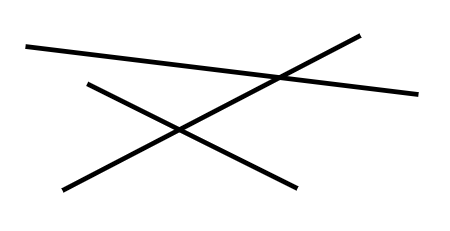
\includegraphics[width=0.4\textwidth]{data/zamiatanie_wariant2_kontrprzyklad.png}
	\caption{  }
	\label{fig:zamiatanie_kontrprzyklad_wariant2}
\end{figure}

\begin{algorithm}[H]
	\caption{Znajdowanie wszystkich punktów przecięcia}
	\begin{algorithmic}[1]
		\Procedure{FindIntersectingPoints}{$S$ -- zbiór odcinków spełniający założenia}
		\State $X \gets$ \textit{zdarzenia} dla każdego punktu $p$ będącego
		końcem pewnego $s \in S$
		\State $Y \gets \emptyset$
		\State Niech $P$ to pusty \textbf{zbiór} punktów
		\While{$X \not = \emptyset$}
		\State \textit{zdarzenie} = $X.$findfirst()
		\State przez $s$ i $p$ oznaczamy
		kolejno odcinek oraz punkt utożsamiony ze \textit{zdarzeniem} w przypadku,
		kiedy $p$ jest początkiem lub końcem jakiegoś odcinka
		\State w przeciwnym przypadku przez $s_1, s_2$ i $p$ oznaczmy kolejno odcinki przecinające się (kolejno dolny i górny)
		oraz ich punkt przecięcia utoższamione ze \textit{zdarzeniem}
		\If{$p$ jest początkiem odcinika $s$}
		\If{$s$ przecina się z $Y$.above($s$) lub z $Y$.below($s$) oraz $x$-owa współrzędna tego przecięcia jest większa niż $p_x$}
		\State Dodaj do $X$ \textit{zdarzenie} zawierające $s$, $Y$.above($s$)
		albo $Y$.below($s$) (zawsze będzie tylko jeden z nich z założenia o braku pionowych odcinków) oraz ich punkt przecięcia
		\EndIf
		\ElsIf{$p$ jest końcem odcinka $s$}
		\If{$Y$.above($s$) przecina się z $Y$.below($s$) oraz $x$-owa współrzędna tego przecięcia jest większa niż $p_x$}
		\State Dodaj do $X$ \textit{zdarzenie} zawierające $Y$.above($s$), $Y$.below($s$) oraz ich punkt przecięcia  
		\EndIf
		\Else
		\State $P \gets P + \{p\}$
		\State $Y$.interchange($s_1$, $s_2$)
		\If{$s_1$ przecina się z $Y$.above($s_1$) oraz $x$-owa współrzędna tego przecięcia jest większa niż $p_x$}
		\State Dodaj do $X$ \textit{zdarzenie} zawierające $s_1$, $Y$.above($s_1$) oraz ich punkt przecięcia
		\EndIf
		\If{$s_2$ przecina się z $Y$.below($s_2$) oraz $x$-owa współrzędna tego przecięcia jest większa niż $p_x$}
		\State Dodaj do $X$ \textit{zdarzenie} zawierające $s_2$, $Y$.below($s_2$) oraz ich punkt przecięcia
		\EndIf
		\EndIf
		\EndWhile
		\State \Return $P$
		\EndProcedure
	\end{algorithmic}
	\label{HasIntersectingSegments2}
\end{algorithm}

Warto zwrócić uwagę na to, że dodajemy zdarzenie, tylko wtedy, kiedy
$x$-owa współrzędna tego przecięcia jest większa niż $p_x$, gdybyśmy tego nie zrobili
pojawią się przypadki, w których będziemy badali dwukrotnie ten sam punkt, co 
może sprawiać problemy implementacyjne.

\subsection{}

